\item Determinar si existe $t\in\R$ tal que los vectores $(t - 1, 0, 1), (t, 1, 2)$ y $(-1, 1, -1)$ sean linealmente independientes.
    \begin{mdframed}[style=s]
        Para que los 3 vectores sean linealmente independientes, se debe cumplir que 
        \begin{center}
            $\alpha(t-1,0,1)+\beta(t,1,2)+\gamma(-1,1,-1)=\vec{0}\Leftrightarrow \alpha=\beta=\gamma=0$\\
            $\begin{cases}
                \alpha(t-1)+\beta t-\gamma=0\\
                \beta+\gamma=0\\
                \alpha+2\beta-\gamma=0
            \end{cases}\to\begin{cases}
                -3\beta(t-1)+\beta t+\beta=0\\
                \beta=-\gamma\\
                \alpha=-3\beta
            \end{cases}\to\beta(4-2t)=0$
        \end{center}
        Eligiendo $t=2$, tengo que $-3(t-1,0,1)+(t,1,2)-(-1,1,-1)=(0,0,0)$, con lo cual, los vectores son linealmente dependientes (ver Figura 4), pero si elijo cualquier otro $t$, entonces $\beta$ tiene que ser 0 y lo mismo sucede con los otros escalares. Por lo tanto, con $t\neq 2$ los vectores son li y dejan de generar sólo un plano para generar todo $\R^3$.
        \begin{center}
            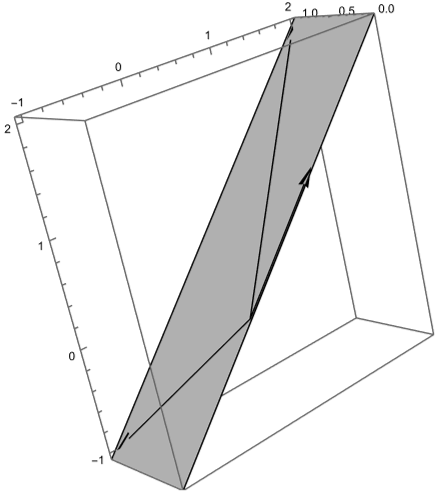
\includegraphics[width=0.28\textwidth]{Ej3.png}\\
            Figura 4. Vectores y plano que se genera con $t=2$
        \end{center}
    \end{mdframed}